%!TEX root = ../../dissertation.tex
%%%%%%%%%%%%%%%%%%%%%%%%%%%%%%%%%%%%%%%%%%%%%%%%%%%%%%%%%%%%%%%%%%%%%%%%%%%%%%%%
\subsection{Cross-Layer Information Exchange}
\label{c5:sec:crosslayerhinting}

The Internet has its historic roots deep in wired networks with a slim and well-defined network stack represented by the \gls{ISO}/\gls{OSI} or \gls{TCP}/gls{IP} model. These layers are isolated against each other. Only predefined information exchange points, or \gls{osiSAP}, at the layer borders allow for vertical communication. A typical wired Internet environment consists of either an Ethernet or other access technologies, e.g., \gls{DSL} or \gls{DOCSIS}, at the physical and link layers or \gls{PON} with \gls{TCP}/\gls{IP} following atop.

Application layer protocols often implicitly rely on the presence and characteristics of specific lower layer protocols. Through the layer isolation no application can precisely know or even control the current state of the lower layers. Nonetheless, they make assumptions on the composition and behavior of the lower layers and plan their work accordingly. 

But the access technology diversity has strongly increased through the advent of wireless technologies, and past behavioral patterns may not be applicable any more today. The protocols used for the radio transmissions behave very differently when compared to Ethernet and assumptions made by higher layers may not hold any more. Examples for this were given in the in the discussion of the stack's influences in Section~\ref{c5:sec:stack-influences}.

It would be very desirable for transport and application layer mechanisms to be able to understand this and cope with these effects. The term \textit{cross-layer interactions} or \textit{information exchange} subsumes these approaches. Specific information from one layer is made available to other interested layers and can even skip intermediate layers.

\begin{figure}[htb]
	\centering
	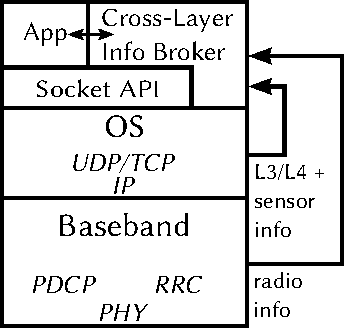
\includegraphics{images/cross-layer-model.pdf}
	\caption{Model and architecture of the proposed cross-layer information exchange.}
\label{c5:fig:crosslayer-model}
\end{figure}

Figure~\ref{c5:fig:crosslayer-model} illustrates this concept with the example of a mobile device. In a fully isolated model, no information would be passed from the baseband to the \gls{os} and the applications. In the cross-layer model certain information would be permitted to pass through. A broker would be responsible to collect information from several sources and layers and make it available to any interested application in a concise manner.

Especially the \gls{3G} mobile layers keep a lot of information, that could be potentially interesting and used in benefit for applications and the user experience.This could include:

\begin{itemize}
	\item Information on the occurrence of a horizontal handover.
	\item Information on neighboring cells and predictions when a handover is most probable to occur.
	\item Information on the occurrence of a vertical handover and thereby changes in the active network stack, e.g., to the WiFi layers.
	\item Information on the current signal strength, bit error rate, and throughput.
	\item More detailed mobility information, including current location and travel speed in relation to base station positioning and availability.
\end{itemize}

In addition to information flow, a path for control flow could also be envisioned. Herein, applications could directly influence the decision making and policies of the lower layers and adapt them to their personal needs.

The impact of a simple unidirectional information flow on the layering mechanisms is suggested to be rather low. Only explicit and specific information is revealed keeping most of the isolation intact. A bidirectional control flow could soften up the isolation and have adverse side-effects. Either way, when implementing any kind of cross-layer exchange, one always has to keep a close look on the resulting consequences. Breaches in the isolation could unintentionally leak network state that could be exploited by malicious parties in any number of unforeseeable ways. Therefore, handling this plays an important role in cross-layer research.

The next sections describe related and similar approaches in the literature and then give some concrete examples on how cross-layer information can be facilitated to the benefit of applications. The cross-layer work is based on a proposal for a FWF~\footnote{Fonds zur Förderung der wissenschaftlichen Forschung, \url{http://www.fwf.ac.at/}} stand-alone project submitted in October 2014 \todo{replace with actual date}. Thus, only initial ideas and planned future work is described.

%%
% ! <-- !
\subsubsection{Related Cross-Layer Approaches}

The idea of exchanging information between layers is not a particularly new one. Some specific ideas have been implemented a long time ago.

Most well known is probably \gls{ECN}~\cite{rfc3168}. Here, the \gls{IP} layer of intermediate hops can signal the end nodes' \gls{TCP} layer that congestion is occurring and \gls{TCP} does not need to wait for implicit congestion signals, e.g., duplicate acknowledgments or timeouts. However, \gls{ECN} is disabled in almost every implementation as it lead to numerous problems and triggered bugs\footnote{\url{http://lkml.iu.edu//hypermail/linux/kernel/0009.1/0329.html}}. This is a risk that many cross-layer attempts may face.

While cross-layer typically implies a solely \textit{vertical} exchange flow there can also be \textit{horizontal} components present.
\gls{DLEP}~\cite{ietf2013dlepdraft} is such an example of a \textit{diagonal} flow, providing information of a lower layer of one entity to a higher layer at another node.
The \gls{DLEP}~\cite{ietf2013dlepdraft} protocol provides information available only to the (external) wireless modem or other interfaces to the routing entity of a node upon which it can act. Link characteristics such as bandwidth, latency, connection status, or information regarding neighbors can be requested.


Though, horizontal information flow is more than often an indication of \textit{centralization} (also called \textit{network-assisted} or \textit{managed}) as apposed to purely vertical \textit{distributed} approaches.




But most cross-layer approaches did not leave the proposal stage. 



Cross-Layer for other stacks: 
SATSIX cross-layer architecture \cite{4656786}


\begin{itemize}
	\item Cross-layer design optimizations in wireless protocol stacks \cite{Raisinghani2004720}
	\item ECLAIR: An efficient cross layer architecture for wireless protocol stacks \cite{raisinghani2004eclair}
	\item Still no implementation of ECLAIR: ``Cross-layer feedback architecture for mobile device protocol stacks'' \cite{1580937}
	\item A multi-layer mobility management architecture using cross-layer signalling interactions\cite{wang2003multi}
	\item Seamless Mobility in Heterogeneous Wireless Networks \cite{zarai2010seamless}
	\item Radio resource management in emerging heterogeneous wireless networks \cite{Piamrat20111066}
	\item Improved community network node design using a DLEP based radio-to-router interface \cite{6379143}
	\item Cross-layer signalling for next-generation wireless systems \cite{1200522}
	\item Cross-layer design for wireless networks \cite{1235598}
	\item A cautionary perspective on cross-layer design \cite{1404568}
	\item User-centric mobility management for multimedia content access \cite{bolla2011usercentric}
	\item Socketless \gls{TCP} --- an end to end handover solution \cite{1635680}
	\item mostly routing protocol optimization oriented ``A cross layer based QoS model for wireless and mobile ad hoc networks'' \cite{krishna2007cross}
	\item SmoothIT mechanisms; lower layer elements provide information to higher layers, overlays\footnote{\url{http://www.smoothit.org}}  \cite{oechsner2009pushing}
	\item ``Mobility Awareness'' \cite{hummel2010mobilitaet} PMLAR (Predictive mobility and location-aware routing protocol in mobile ad hoc networks)
	\item Automatic Multi-interface Management Through Profile Handling \cite{Bonnin:2009:AMM:1503496.1503498}
	\item A ubiquitous mobile communication architecture for next-generation heterogeneous wireless systems \cite{1452832} (supposed to propose a function that determines the best handover initiation time in order to avoid early or late initiations)
	\item Optimized video streaming over 802.11 by cross-layer signaling \cite{1580941}

 	\item Modem Link Properties Advertisement Protocol\footnote{\url{https://tools.ietf.org/html/draft-ivancic-mobopts-modemlpa-01}}

\end{itemize}


%LCP Link Control Protocol, PPP extension RFCs \cite{rfc1570,rfc1661}
%LISP and other mobility approaches \cite{rfc6830}

% Conceptually similar to cross-layer interactions is the family of dynamic radio resource management techniques. These control many properties concerning radio resources. 
% Radio Resource Management RRM
% 		\begin{itemize}
% 			\item resource monitoring, decision making, decision enforcement
% 			\item choose available wireless interfaces  best suited for a specific task
% 			\item rudimentary implementations in mobile OSs
% 		\end{itemize}
%	IEEE 802.21 cooperative handovers, but with required network support

%%
\subsubsection{Application Usage and Adaptation Scenarios}


 E.g., \gls{TCP} retransmissions and congestion control could be adjusted in the course of understanding this.

Furthermore, traffic could be avoided during cell handover occurrences. This would require cross-layer cooperation and an awareness of the application when an handover is supposed to occur. The application then could schedule its traffic accordingly. Traffic falling into a handover is subject to especially high latency and loss because the mobile network acts as a mobility anchor which needs to internally reroute incoming traffic to the mobile device's new position. \gls{HTTP} traffic is especially suited to this scheduling behavior because of its statelessness and consistence of small objects that can be requested and transferred independently.

Today's mobile networks are all of a cellular design. A device that moves from one cell to the other has to perform a so-called handover. During this process the device is deregistered in one cell and registered in the new one. All network traffic currently in flight has to be rerouted or relayed to the device's new location. 
Although seemingly transparent to the device's application, adverse side effects can occur during a handover, including an increase and variability of latency. 

Mobility support today always means network assisted mobility. Typically, the network decides the best possible mobility strategy from its point of view and provides infrastructure to support seamless handovers in the form of mobility anchor nodes. However, the device is actually in a very unique position, as it knows a great deal more about its traffic mix, its currently running applications and its user than the network ever could and should.
Unfortunately, most of this information remains unused, as today's network infrastructures and lower layer protocol stacks provide only very slim changes to exert control over decisions regarding the device.

Nonetheless, a lot could still be done when providing the device's operating system and application ecosystem with a simple bidirectional pathway for vertical information and control flow across network protocol layers and to other low-level systems. This work aims to do just that by providing a generic interface and exchange protocol for any kind of information relevant to an application's decision making process. With this meaningful actions and reactions of individual layers can be defined and tested. Possible use cases are provided in the next section.

Still, one has also to keep in mind, that layering and encapsulation is there for a reason and violating this is a rather risky undertaking. However, we do not think that our approach actually violates these basic principles and only extends on the ways one can communicate and interact with all individual layers without changing anything in them.


	% - Research objectives
	% 	- Bidirectional vertical information and control flow on the performance of the individual layers
	% 		- Definition of generic interfaces
	% 		- Definition of a protocol (including information types, etc.)
	% 	- Definition of meaningful actions/reactions on the individual layers (e.g. adaptation of real-time communication data sources or changes in resource allocation)

		


\begin{itemize}
	\item Video/Voice calls that notify the other party, that interruptions are expected to occur.

	\item Using current location data and movement patterns/predictions to improve cell selections and initiate horizontal and vertical handovers to a time suitable for the device and running applications.

	\begin{figure}[htb]
	        \centering
	        \begin{subfigure}[b]{0.90\textwidth}
	            \centering
				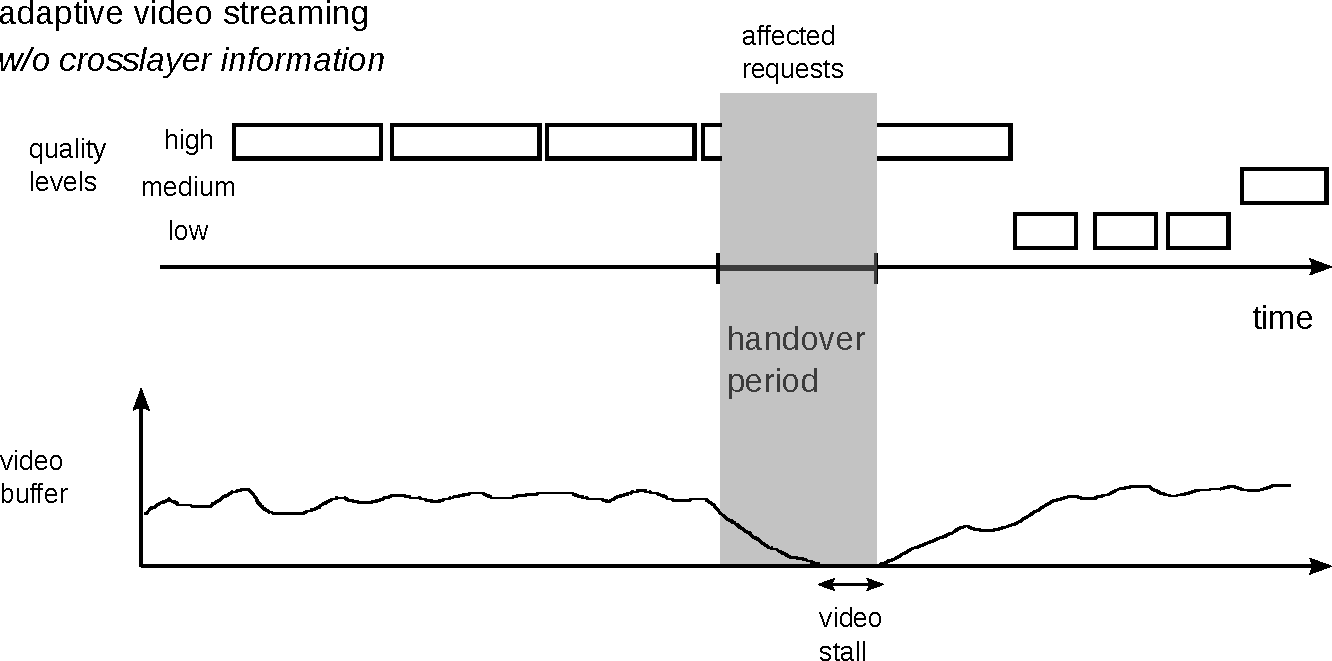
\includegraphics[width=\textwidth]{images/adaptive-streaming-no-cl.pdf}
				\caption{Stalling occurs without handover hinting.}
				\label{c5:fig:streaming-hinting-no-cl}
	        \end{subfigure}%

	        \begin{subfigure}[b]{0.90\textwidth}
				\centering
				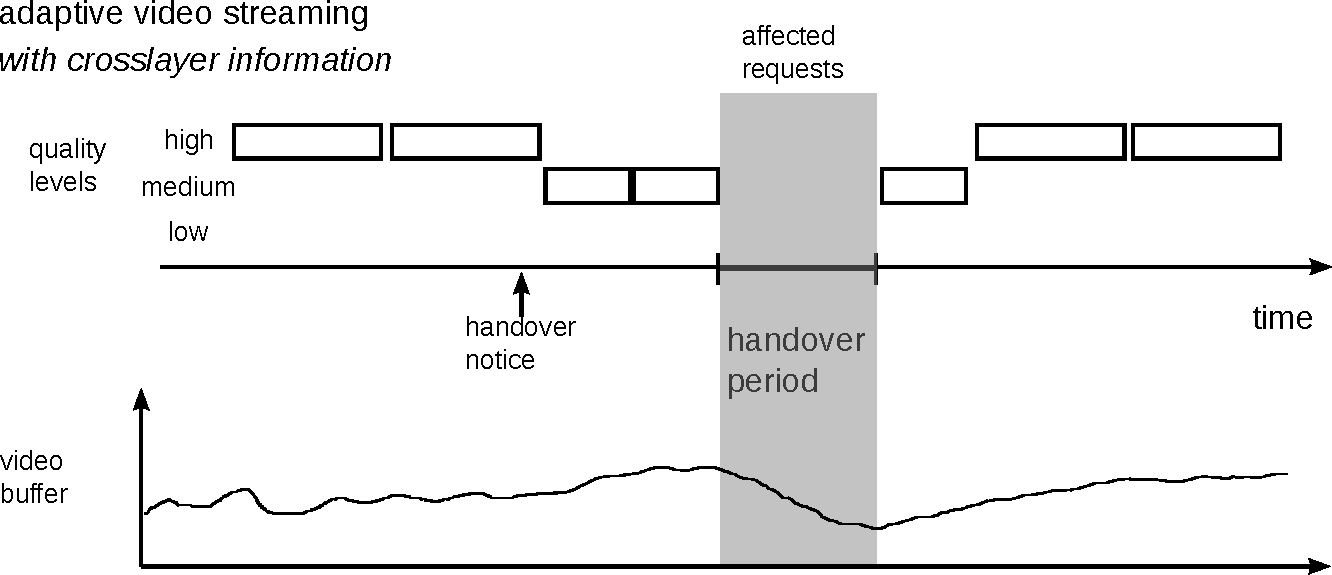
\includegraphics[width=\textwidth]{images/adaptive-streaming-cl.pdf}
				\caption{Stalling can be prevented by hinting and proactively filling the playback buffer.}
				\label{c5:fig:streaming-hinting-cl}
			   \end{subfigure}%
	 \caption{Mockup of handover prediction and hinting for adaptive streaming and thus avoiding playback stalls.}
	\label{c5:fig:streaming-hinting}
	\end{figure}

	\item An adaptive streaming video application increases its video buffer when a shortly upcoming handover is announced to survive the service outage. This can be achieved by an increased rate of segment retrieval and a reduction in segment quality. The goal is to avoid any possible playback stalls due to the handover. Figure~\ref{c5:fig:streaming-hinting} demonstrates this circumstance.

	\begin{figure}[htb]
	        \centering
	        \begin{subfigure}[b]{0.90\textwidth}
	            \centering
				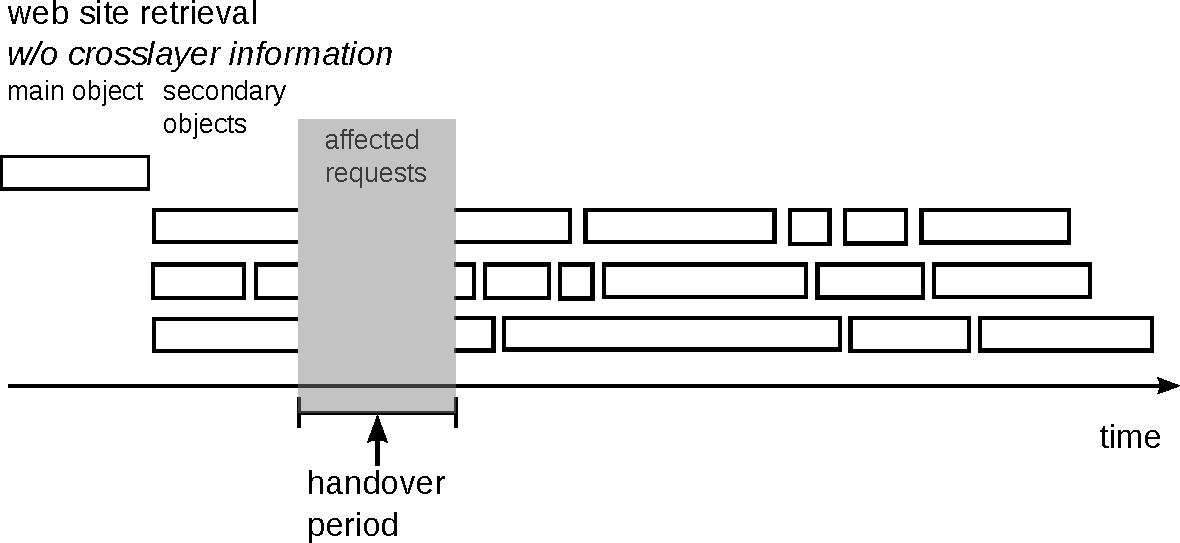
\includegraphics[width=\textwidth]{images/http-reorder-no-cl.pdf}
				\caption{The handover will block currently active object transmissions, page display will be delayed.}
				\label{c5:fig:http-reorder-no-cl}
	        \end{subfigure}%

	        \begin{subfigure}[b]{0.90\textwidth}
				\centering
				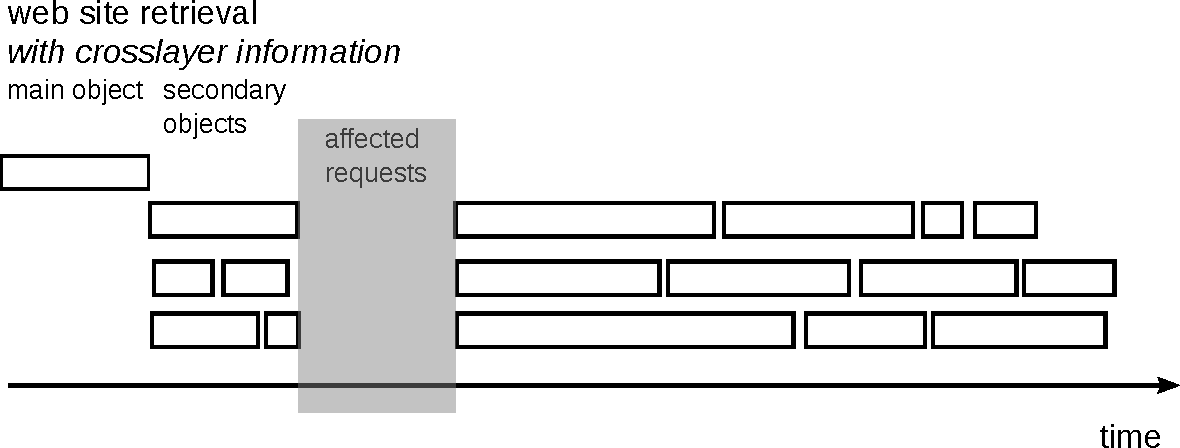
\includegraphics[width=\textwidth]{images/http-reorder-cl.pdf}
				\caption{The browser reorders the objects to be retrieved and avoids any transmissions during the indicated handover period.}
				\label{c5:fig:http-reorder-cl}
			   \end{subfigure}%
	 \caption{Mock-up of \gls{HTTP} reordering with handover awareness.}
	\label{c5:fig:http-reorder}
	\end{figure}

	\item Enable applications to adapt themselves to the conditions currently experienced by the networking stack and its sensors. For example, a Web browser could reorder its Website object requests to avoid sending any requests during handover periods and experience additional delay as seen in Figure~\ref{c5:fig:http-reorder}.

	\item A cross-layer enabled device can also offer a wide range of policy choices to its applications or even directly to the user. An example rule could be: ``Do not handover to a stationary WiFi from 3G when moving faster than 50km/h, only to in-vehicle WiFi.'' or ``Avoid any vertical handover, which would interrupt my service for a long time, while this VoIP call is running.''

\end{itemize}

Example Benefits

Put into relation:

\begin{itemize}
	\item frequency of handovers / distance/density of radio towers vs scenario traveling speed
	\item bit-length of streaming segments, typical transmission speed
	\item typical video length and number of segments
	\item derive number of interruptions in segments due to handovers
	\item estimate typical handover/mobility duration and service interruption time per event
	\item sum it up and compare to crosslayer information or even application layer handover decision
\end{itemize}


\subsubsection{Proposal}

The Implementation:
\begin{itemize}
	\item Userspace daemon that collects information from kernelspace protocol implementations and sensors and provides them to all applications.
	\item shared bus control/information system, instead of explicit comm; signaling only to interested parties
	\item provide common interface also to all available sensors and layer 1 and 2 network information and control (similar to Android)
	\item IPC message bus, possibly D-Bus\footnote{\url{http://www.freedesktop.org/wiki/Software/dbus/}} based
	\item Could extend NetworkManager\footnote{\url{https://wiki.gnome.org/Projects/NetworkManager}}, some functionality is already provided there

\end{itemize}

The process:
\begin{itemize}
\item Tell Transport/Application the expected time till handover / time of uninterrupted service
\item Tell Transport/App expected connection parameters (latency, BW, ...)
\item Application selects \gls{DASH} stream appropriate to parameters
\item Application reorders \gls{HTTP} GETs so that large GETs are not interrupted
\item Application stops transfers when handover is about to occur
\item Layer 1/2 gives a list of possible handovers to Application
\item Application selects (better: suggests) handover which fits best and reorders accordingly
\end{itemize}


\begin{itemize}
	\item investigate how much information is exposed and what can already be done
	\item Analysis of data traces and realistic simulations in order to capture in detail the unwanted phenomena
	\item Verify the suitability of the State-of-the-Art algorithms and protocols which address this problem
\end{itemize}


% influence of signaling plane and core network elements - scaling
%This can apply to, e.g., reliability, frame sizing and fragmenting, and latency amounting to undesired effects on higher-layer traffic. 